\chapter{Data Collection}\label{ch:data}
You can't make bricks without straw. Data is necessary to make inference, and
since it's usually only possible to get a sample from the entire population,
it is important that the sample represents the population faithfully. This chapter 
discusses the problems that may arise when a sample is not representative
of the population, and how this may lead to entirely invalid conclusions.

\hypertarget{ch:data}{%
\section{Representative sample}\label{representative}}
\hypertarget{ch:data}{%
\subsection{Definitions of key terms}\label{keyterms}}
First, let's introduce some terminology. A \emph{population} is the set of 
individuals (\emph{subjects}) which we're interested in studying. Subjects may be 
people, mice, or devices produced in a factory, just to name a few examples. 

A \emph{sample} is a subset of the population. The sample is said to be
\emph{representative} if it reflects the characteristics of the population.
For example, if in the United States the proportion of females is approximately 50\%,
then a sample taken from this population should also have approximately 50\% females
in order to be considered representative.
This is important because a main goal of statistical data science is to use the
smaller sample to draw conclusions on the population.
We saw in chapter \ref{ch:llnclt} that the law of large numbers and the central limit
theorem guarantee that if the sample is representative of the entire population,
then our estimates can be trusted with a certain degree of confidence,
and the largest the sample, the more confident we are about the estimate
and the conclusions that we can draw from it.

However, if the sample doesn't faithfully represent the population, then no matter
how large the sample is, the results can't be trusted. When the quantity we want
to estimate and reason about is estimated based on a non-representative sample,
we get a \emph{biased} estimator. By bias we mean that the obtained estimate
is not a good approximation of the true value, and it doesn't improve when we
take a larger sample.


Let's illustrate the notions of population, sample, and bias through simulations.
Assume that for a group of people,  weight and height have a linear relationship
\begin{equation}
  \label{eq:weightheight}
  \text{weight} = -194.49 + 5.30*\text{height}\,.
\end{equation}

However, because people have different activity levels and different diets, each
person's weight is a little different than the one predicted by Equation (\ref{eq:weightheight}).
We write the weight as a function of height using an equation that includes this 
random `noise', by adding
a non-deterministic (\emph{stochastic}) term, denoted by $\text{Error}$:
\begin{equation}
  \label{eq:weightheight}
  \text{weight} = -194.49 + 5.30*\text{height} + \text{Error},
\end{equation}
where, in our simulation, the Error has a normal distribution with mean zero and standard deviation
23.26. We simulate such a population with $N=500$ people and plot their weights
against heights using the following code. The result is given in
Figure~\ref{fig:representativesample} (a), where, in addition to the 
`noisy' data of the population we also show the true (linear)
relationship between height and weight.

\showChunk{R}{Code/datacollect-goodbadsample.R}{BIASgbs1}

Now we use the following code to uniformly and randomly select $n=50$ people as
a sample from the population and mark the selected people in
Figure~\ref{fig:representativesample} (b) using the dark trinagles. The \code{sample()} function
is used to draw a \emph{simple random sample (SRS)} of size \code{n}
from the population of size \code{N}. SRS means that every subject in
the population has an equal probability of being selected into the sample.
We see that the smaller sample of
$n=50$ (depicted by dark triangles) gives a similar relationship between weight 
and height as observed in the
larger population of $N=500$. Here the sample is a representative one. 

\showChunk{R}{Code/datacollect-goodbadsample.R}{BIASgbs2}

Now, let's assume that the way to take a sample depends on both the weights and
heights in the population. We create a function of weight and height
and use it to 
determine the probability of including a person in the sample. The following code
uses this way to take a sample and plot it in
Figure~\ref{fig:representativesample} (c).
In the code, \wingding{1} and \wingding{2} create a variable \code{w} that
depends on the weight and height of the people in the population; and
\wingding{3} uses the variable \code{w} to decide the probability of including a
person into the sample. The larger the value of \code{w}, the higher the
probability of including the person in the sample. The exact way we 
obtain \code{w} in this example is not important. What's important is
that the selection of an individual into the sample is \emph{not random}. 
When the probability of drawing a subject into the sample depends on his/her
height, weight, or both, then the sample is no longer representative and
as such, it doesn't retain the properties of the population. 
\showChunk{R}{Code/datacollect-goodbadsample.R}{BIASgbs3}

In Figure~\ref{fig:representativesample} (c) you can see that the relationship
between the height and the weight in the population is along the line
with slope 5.3, but in the sample (dark red dots) the relationship between 
the two variables is more or less along a vertical line with mean height of
about 70.

\runR{Code/datacollect-goodbadsample.R}{datacollect-goodbadsample}
% \showCode{R}{Code/datacollect-goodbadsample.R}
% \includeOutput{datacollect-goodbadsample}

\begin{figure}
  \centering
    \begin{subfigure}{0.32\textwidth}
      \includegraphics[width=\textwidth]{images/chapter_6/population.pdf}
      \caption{Population}
    \end{subfigure}
  \begin{subfigure}{0.32\textwidth}
      \includegraphics[width=\textwidth]{images/chapter_6/representSample.pdf}
      \caption{Representative sample}
  \end{subfigure}
  \begin{subfigure}{0.32\textwidth}
      \includegraphics[width=\textwidth]{images/chapter_6/biasedSample.pdf}
      \caption{Biased sample}
  \end{subfigure}
  \caption{An illustration of representative and non-representative samples}
  \label{fig:representativesample}
\end{figure}

To see the effect of a biased sample, let's look at the variance of height
in the population, and in the two samples. We can use the following code:
\showChunk{R}{Code/datacollect-goodbadsample.R}{BIASgbs4}

The variance in the population is called \code{var0} in the code and it's equal to
\inlnR{```cat(var0)```}[var0]. In the first (simple random) sample the
variance is called \code{var1} and is equal to \inlnR{```cat(var1)```}[var1], which is very close to the
actual variance in the population (the difference is \inlnR{```cat(var1-var0)```} [diff01]),
but in the second (biased) sample, the variance of height is much smaller: \code{var2} 
is 
\inlnR{```cat(var2)```}[var2].

\hypertarget{ch:data}{%
\subsection{A representative sample is more important than a larger sample}\label{representative}}

\begin{example}[The 1936 Literary Digest Poll, \citep{darkdata_ch2}]
 For the 1936 presidential election, the Literary Digest poll was one of the
largest and most expensive polls with a sample size of around 2.4 million
people. Based on every telephone directory in the United States, lists of
magazine subscribers, rosters of clubs and associations, and other sources, a
mailing list of about 10 million names was created. Every name on this list was
mailed a mock ballot and asked to return the marked ballot to the magazine. The
Literary Digest predicted that Alfred Landon would get 57\% of the vote against
Franklin D. Roosevelt's 43\%, while the actual results were 38\% for Landon
against 62\% for Roosevelt. At the same time, George Gallup was able to predict
a victory for Roosevelt using a much smaller sample of about 50,000 people.

There were two major flaws in the way Literary Digest collect the sample: 1) The
mailing list only contained some subgroups of people in the U.S. For example,
telephone service was not commonly available in the 1930s. Similarly, most people might not
belong to any club or other associations. So, the Literary Digest poll 
reached only the relatively affluent part of the population. 
2) People on the list decided if they
would return the ballot to the magazine, so the resulting sample is a
``volunteer'' sample.

As a result, the data collection method of Literary Digest
did not produce a representative sample of the U.S. population and thus 
resulted in a biased estimate and a misleading conclusion.  In the next section,
we elaborate on different types and sources of bias. While preventing
all sources of bias may be challenging, the only chance we have if we want
to eliminate any bias from our sample (and we do!) is to be aware of the potential
pitfalls.
\end{example}

\subsection{Randomized control trials vs. observational studies}
The gold standard in data collection is to perform a \emph{randomized control trial} (RCT).
This can only be done if we can pre-plan our experiment, and we know in advance
what data needs to be collected. The typical examples are in medical experiments,
where the outcome that we intend to measure (e.g., blood pressure) is believed to
be associated with a treatment (e.g., a new drug.)
There may be multiple factors affecting the outcome (or at least, that could affect it).
For example, we may have a reason to think that age, sex, body mass index (BMI),
or other things are related to one's blood pressure.
In a randomized control trial we can get a representative sample of the population,
and randomly assign each individual to one of the treatments. With randomization
we end up with comparable groups of individuals. For example, if we are testing
two new drugs, and one old drug, then there are three treatment groups and in each one
we have approximately the same age distribution, the same proportions of females,
the same distribution of BMI, etc.

Then, the comparison between the three types of treatments is meaningful,
and we can use it to draw conclusions about the effect of the treatment (drug, in our example)
on the outcome (blood pressure). Because, if other than the treatment,
the subpopulations in all groups are identical, then if there is a difference in
the outcome between the groups, then it must be due to the one thing that separates the
groups.

The \emph{control} part in RCT means that one of the treatment groups is our baseline,
and we compare all the other types of treatments to it. In our example, the old drug's
effect on blood pressure is known, and we want to know if the new drugs give better
results in controlling blood pressure.

Similarly, suppose that we have a number of workout regimes and we want to
see which one gives the best results in, say, body weight, or endurance. Then
we could randomize the subjects in our sample, and divide them into treatment
groups, one of which is `no training'. This is then our baseline level---we can check
which (if any) of the training regimes is better than the inactive group.

Unfortunately, running an RCT is not always possible. First, it may be hard or expensive
to gather the sample. For example, drug development is expensive, because
it takes a long time and requires expensive materials and equipment,
as well as many experts. It is also hard to collect the data because patients have
to be recruited and monitored, and the whole process has to be vetted by the
authorities, in order to ensure that it is done properly and fairly. 
Second, it may be impossible to randomize participants into groups
that only differ in the treatment that they receive. This can be, for example, due to
ethical reasons, especially when human subjects are considered.
For example, if we want to check the effect of smoking on the risk of getting lung cancer,
we can't assign people to the smoking group, since we have reason to believe that
this is harmful.
Third, there may be many factors that \emph{could be} related to the outcome. If we want
proper randomization, the groups have to have the same distribution for all these
factors, which means that the sample size we must collect grows quickly when we
add multiple factors. Finally, even if we have the time and budget to perform the RCT, 
and we can randomize the subjects properly and ethically, there may still be factors
that we haven't considered, but are important. Any missing variable (a factor that
may affect the outcome) can make it impossible to draw conclusions about the
treatment effect. After all, without the missing data, we can never tell for sure if
the observed differences between the groups is due to the treatments, or to the
missing factors!

Most of the time, the data that's available for analysis is not from RCTs, but from
\emph{observational studies}. These are typically much easier to collect, but they don't
guarantee proper randomization, and that may lead to biased results. 
For example, we may want to look at the effect of education on future income.
We can conduct a survey and ask people how many years of schooling they had
and what's their current salary, and possibly ask them about other factors such as age,
sex, what they majored in (if they went to college), and so on. The data collected 
from this survey is observational in nature---none of the participants was assigned randomly to 
any particular group. They were either lucky or unlucky enough to have a certain 
socioeconomic background, or they chose where to go to school.
So, in such surveys (which are much easier and cheaper to collect than RCTs),
individuals are not randomly assigned to groups by the people designing the experiment,
but rather, they can \emph{select} their own group. 


Whenever we analyze data, we must know how it was collected. Was it through a randomized 
control trial, or is it just data that came from an observational study? Conclusions
from the former can be much stronger, in the sense that they allow us to establish
cause and effect relationship. But, as we said, most of the data that we encounter
doesn't come from a RCT. In these cases, we must be careful when we draw conclusions.
Usually, we can only make statements about \emph{associations} between variables,
but not much (if at all) about causality.




\hypertarget{ch:data}{%
\section{Types of data problems}}
In this section we introduce a few types of data collection problems that lead to
biased samples. 
David Hand, in his book \emph{Dark Data} \citep{darkdata_ch2} discusses 15 different
types of `dark data' -- data that we don't observe, and by ignoring its existence we 
are lead to wrong (potentially disastrous) conclusions. 
We will demonstrate some of these data problems in this chapter.

\subsection{Berkson's bias}\label{berkson-bias}
In his book, \textit{How Not to Be Wrong: The Power of Mathematical Thinking}, 
Jordan Ellenberg poses the question:
 `\textit{Why are handsome men such jerks?}' \citep{ellenberg2015not}.
%https://medium.com/@penguinpress/why-are-handsome-men-such-jerks-f385a46d314f

Are they? Similarly, you may have seen articles which focus on ``popular books whose 
movie adaptations were not-so-good'', and you may get the impression that 
Hollywood ruins good books. But, is it true?
 % (e.g., \href{https://www.yardbarker.com/entertainment/articles/popular_books_that_were_made_into_terrible_movies/s1__29971472}{here})
  % \href{https://www.cinelinx.com/movie-news/movie-stuff/bad-books-that-made-great-films/}{here}).

You may have heard similar common impressions, such as
that pretty girls are meaner, and more talented people are less attractive.

What is the source of these (false) impressions? The answer is that 
they usually result from a type of \emph{selection bias}, where the data
are not collected at random and some items have a higher or lower probability
of being included in the sample. The particular form of bias in this case has a name,
and it's called \emph{Berkson's bias}. Let's start with an example to explain.

\begin{example}[Stamps display]
  Suppose you have 1,000 postage stamps: 300 are pretty, 100 are rare, and 30 are
  both pretty and rare. Is a rare stamp more likely to be pretty?  Now you want
  to show some of your stamps to your friends. You probably want to show them
  the pretty ones and the rare ones. Let's say you only show the 370 stamps which
  are either pretty or rare to your friends. Based on what your friends
  observe, will they conclude that a rare stamp more likely to be pretty?
\end{example}

Let's calculate some numbers to see the answer. For all the stamps, the
probability that a stamp is pretty is 300/1000=0.3; for rare stamps, the
probability that a stamp is pretty is 30/100=0.3. Thus, a rare stamp is as
likely to be pretty as in the entire collection.

For the stamps you showed your friends, the probability that a stamp is pretty is
300/370=0.81; for rare stamps, the probability that a stamp is pretty is
30/100=0.3. Your friends' conclusion would be: a rare stamp is much less likely
to be pretty!

The reason for their incorrect conclusion is that the 370 stumps are not a
representative sample of all the stamps you have. They were picked
specifically to impress, so the stamps that were neither rare, nor pretty
are not represented in the sample. This means that this sample is biased.
As showed in the Venn diagram in Figure~\ref{fig:stamps}, the area of the red
circle is a small proportion (0.3) of the area of the rectangle, while it is a
large proportion (0.81) of the area of the colored region (the biased sample). 

\begin{figure}[H]
\resizebox{0.6\columnwidth}{!}{%
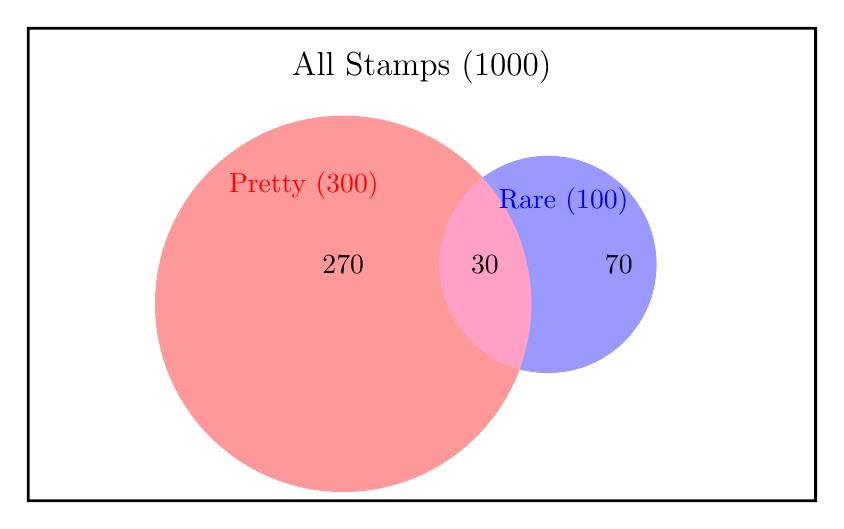
\begin{tikzpicture}
  \begin{scope}[blend group = soft light]
    \draw (-5, 3) rectangle (5, -3);
    \fill[red!40]  (-1, -0.5) circle (2.39);
    \fill[blue!40] (1.6, 0)   circle (1.38);
  \end{scope}
  \node       at (0, 2.5)    {\large All Stamps (1000)};
  \node[red]  at (-1.5, 1)   {Pretty (300)};
  \node[blue] at (1.8, 0.8)  {Rare (100)};
  \node       at (-1, 0)     {270};
  \node       at (2.5, 0)    {70};
  \node       at (0.8, 0)    {30};
\end{tikzpicture}
}
\caption{Venn diagram for the stamps example. The rectangle represents all the
  stamps, the large red circle represents the pretty stamps, and the small blue
  circle represents the rare stamps. The numbers indicate how many stamps are in
  each region.}
  \label{fig:stamps}
\end{figure}

Now let's simulate some data to further illustrate the problem. In this simulation,
we use the ``popular books whose movie adaptations were not-so-good'' example.

\showCode{R}{Code/datacollect-berkson.R} %
\runR{Code/datacollect-berkson.R}{datacollect-berkson} %

In the above code, the goodness of books and movies are drawn independently from a
standard normal distribution (\wingding{1} and \wingding{2}). \wingding{3}
checks if a book is good (better than 90\% of all books) and \wingding{4} checks
if a movie is good (better than 90\% of all movies). A component of the variable
\code{good} in \wingding{5} is \code{TRUE} if the book and/or the movie is good.
Running the above code should give the two figures in Figure~\ref{fig:berkson}
and the following output.
\includeOutput{datacollect-berkson} %

We see from the output and Figure~\ref{fig:berkson} (a) that the correlation between
the goodness of books and the goodness of movies is very close to zero---there
is no linear association between them. However, if we limit our data to inoclude
only movies such that either the book is good, or the movie is good, or both are good, 
and we then look for a linear association between the quality of books and movies,
then there is a clear negative linear relationship, as can be seen in 
Figure~\ref{fig:berkson} (b).


\begin{figure}[H]
  \begin{subfigure}{0.485\textwidth}
    \includegraphics[width=\textwidth]{images/chapter_6/berkson1.pdf}
    \caption{No linear association between goodness of movies and goodness of
      books}
  \end{subfigure}
  \begin{subfigure}{0.485\textwidth}
    \includegraphics[width=\textwidth]{images/chapter_6/berkson2.pdf}
    \caption{Negative linear association for top 10 percent books and/or movies}
  \end{subfigure}
  \caption{Goodness of movies v.s. goodness of books}
  \label{fig:berkson}
\end{figure}

People typically only recommend good books or good movies to other
people, so what we see are only these with the best review. If a book is
bad and the movie based on it is terrible, it's very likely that you ever have
a chance to hear about them. Thus, the impression that Hollywood ruins good books is
false. It's just an impression based on a biased sample. 

The `blank square' in the bottom-left corner of Figure~\ref{fig:berkson} (b), where we see no
points at all, is our \emph{dark data} in this example, and is the source of
our biased result, and the false impression. There are, in fact, many data
points in this region, but we never observe them.
\why{remove this?}
They include some very bad books that were turned into very good movies.
\why{or change it to something like: They include the majority of bad books and bad movies.}

This type of selection bias problem is related to the idea of \emph{conditional probability},
which we discussed in Chapter \ref{ch:probability}. When we calculate probabilities, or
obtain other statistics, our results depend on the  set of possible events. If we limit 
the set of observable events, we should generally expect our selection to have
an impact on our analysis. Only when the selection of the subset is \emph{independent}
of the characteristics of subjects in the population, can we trust the results obtained
from a sample.

\hypertarget{ch:data}{%
\subsection{Survival Bias}\label{survival-bias}}

Survivor bias arises when observations are limited to subjects or objects that
have ``survived'' or successfully completed a particular process, while those
that did not are overlooked. For instance, poorly performing hedge funds often
close and are excluded from indexes, skewing performance analyses. Similarly,
prominent success stories like Facebook dominate the spotlight, overshadowing
the vast majority of failures. Ignoring survivor bias can result in misleading
or even entirely incorrect conclusions, as it fails to account for the unseen
data that play a critical role in understanding the complete picture.

\begin{example}[hit aircraft]
During World War II, aircraft that had returned from missions were examined and
the most-hit areas of the plane are given in
Figure~\ref{fig:survival-bias}. Which areas should the army add armor to
increase the survivorship of the planes?

A direct intuition may suggest to reinforce areas with the most bullet holes
because these are the most hit region. However, the data were collected from the
aircraft that had survived their missions, and if an aircraft was hit and down
it would not be included in the data. If there is a bullet hole in the engine
area or in the cockpit, then it would unlikely that the aircraft could
return. This was actually the reason why the engine and cockpit regions were
almost free of bullet holes. Knowing that the marked dots for bullets holes were
a biased sample and the cause of the bias, we should realized that these regions
with bullet holes could take damage and the aircraft could still fly well enough
to return safely. These regions did not need additional armor. It is the areas
where the returning aircraft were unscathed that need additional armor.
\end{example}

This example shows that ignoring the bias may give a very wrong conclusion. If
we take into account the source of the bias, then we can still obtain valid
result from a biased sample.

\begin{figure}[H]
  \includegraphics[width=.85\textwidth]{images/static/Survivorship-bias.png}
  \caption{Most-hit areas of the returned aircraft. Source: \url{https://en.wikipedia.org/wiki/Survivorship_bias}}
  \label{fig:survival-bias}
\end{figure}

\hypertarget{ch:data}{%
\subsection{Base-Rate Fallacy}\label{base-rate}}

The \emph{base-rate fallacy} is a common source for many misconceptions
and misinterpretations of data. 
Consider the following example. A pet store owner finds that his store was broken into,
and a parakeet was stolen. He calls that police, who find two things on the scene:
they see Teddy walking nearby, looking rather suspicious in their mind (but no parakeet
in his possession), and they find drops
of human blood in the store. They detain Teddy, and send the blood to the lab, and find that 
it's type $B-$. The they get a blood sample from Teddy, and find that
he has that blood type, and they immediately arrest him for the burglary.

What is the probability that Teddy is the burglar?

To answer that, we need a bit more information. Let's say that the pet store is in London.
In the U.K., 2\% of the population has a $B-$ blood type? The test for detecting
blood types is 100\% accurate, so given that Teddy was determined to have
a $B-$ type, we can assume that this is correct.
The prosecutor claims that the probability is 98\%. Let's check if it's true, by simulating data.

In the following code we simulate a population of 1,000 people, of which 2\% 
have Teddy's blood type, $B-$.
We use the \code{sample} function to draw 20 people out of the population
to have blood type $B-$ \wingding{1}. 

\runR{Code/datacollect-baserate.R}{datacollect-baserate}

From these 20 people, we draw one person to be the real perpetrator \wingding{2}.
Then, we check the probability that that person is Teddy \wingding{3}. We run a loop
200 times, representing 200 identical (hypothetical) burglaries, and check
whether the person detained by the police (Teddy) is the real perpetrator.

\showCode{R}{Code/datacollect-baserate.R} %

The number of time that Teddy was, in fact, the perpetrator in those
200 hypothetical burglaries is 
\inlnR{```cat(sum(teddy == perp))```}[teddyperpnum], and since we ran
the simulation 200 times, it means that Teddy was \emph{not}
the perpetrator \inlnR{```cat(100-100*sum(teddy == perp)/length(teddy))```}[teddyperppct]\% of the times!

This so-called base-rate fallacy is also known as the \emph{prosecutor fallacy}.
It's related to Bayes' theorem which we've encountered in Chapter \ref{ch:probability}. 
It's called the base-rate fallacy because we must take into account the
prevalence of the blood type in the entire population. If we don't, and we 
only rely on how accurate the blood type test is, then we reach the
wrong conclusion.

In other words, we must consider not only the probability of getting a
\emph{true positive} result, but we must also consider the probability
of a \emph{false positive} result! 

This scenario happens in different settings. For example, in diagnosing 
a rare disease, getting a positive test result doesn't mean that the person
has the disease. Similar calculations show that, because the disease is rare,
even an accurate test procedure can lead to misleading conclusions (and
in some cases, with severe consequences.)

In his book, David Hand mentions that when a problem like the one we've
just discussed was presented to Harvard medical school students,
over 56\% got the wrong answer because they only considered the
accuracy of a test, and ignored the prevalence of the disease and the
probability of a false positive \citep{darkdata_ch2}.

\hypertarget{ch:data}{%
\subsection{Omitted Variables}\label{omitted-vars}}
Sometimes we just don't know that we're missing critical data. It can be
in the form of base-rate fallacy, where the data we may be ignoring
(unless we're careful) is the prevalence of something in the population,
such as blood type or a disease. In other cases, we may be missing data
because of \emph{selection bias}, where we inadvertently analyze only
a non-random sample, as was the case with Berkson's bias or in the
survival bias story.

If we think of the data as a table in which the rows are subjects (cases) and
the columns are variables---properties of each subject or case, then the previous
examples were all about missing \emph{rows} in the table. When
rows are missing completely at random, we can still get good estimates
and predictions, but if they are missing in some systematic way, then
the results we get can't be trusted. They may be biased and lead to wrong 
conclusions.

In this subsection we consider the case where what we're missing
is \emph{columns} (variables) in the data table.
We've already seen two such examples in previous chapters. The first one
appeared in Chapter \ref{EDA}, Figures \ref{sidebysidebp} and 
\ref{scatter}. There, the variables where \code{x} (e.g., time) and
\code{g} (e.g., the A/C is working or not). We saw that only when we 
considered both variables  \code{x}  and  \code{g}, were we able
to see the real pattern of \code{y} (say, the temperature).

The second example appeared in Chapter \ref{simpsons-paradox}, where we
discussed Simpson's paradox. When we looked at the overall admission rate
to UC  Berkeley, it looked like the rate for women is considerably lower, but when 
we added a variable (the specific departments), the conclusion was quite different,
and in fact, in most departments the admission rate was higher for women.

The trouble with this kind of missing data is that we may never know what's missing!
As we discussed in Chapter \ref{EDA}, we should always try to use plots and tables
to visualize and understand the nature of the data. In the \textcolor{red}{regression} chapter,
we'll see that in some cases we may get hints for missing variables from the so-called
regression diagnostics plots.

\runR{Code/datacollect-omitted.R}{datacollect-omitted}

However, there's no guarantee that we'll be able to identify a missing variable, and
which may lead us to misinterpretations of data. To see it, let's look at another example.
Phil is a realtor who works in a small college town. The college has been around for
a couple of centuries, and is very prestigious. His clients often wonder
why the houses that are farther from the campus cost so much more than the 
ones in walking distance.
Phil collected data and plotted the graph in Figure \ref{fig:omitted},
which shows the square of the distance in miles of houses from the 
campus on the x-axis, and the price (in thousands of dollars) on the 
y-axis. He also added a fitted line, which shows a positive trend.

\begin{figure}[H]
  \includegraphics[width=.6\textwidth]{images/chapter_6/omitted.pdf}
  \caption{The relationship between the square of the distance from a house to the campus, and 
  the house price, in thousands of dollars}
  \label{fig:omitted}
\end{figure}

Phil concludes that, indeed, the farther the house from campus, the more
expensive it is. But surely, many people who work at the university prefer to live 
close by, and have the means to do so, so what could drives the prices of
more remote houses up?

With observational data, it's tempting for Phil (and most people) to find
a way to explain a phenomenon that defies common sense.
For example, Phil may come up with a theory that faculty want to
live away from campus in order to avoid their students. Or, he may 
hypothesize that close to the campus the crime rate may be higher than in the
suburbs. You can probably come up with other plausible explanations.
However, without additional information, they are just guesses. These guesses
may seem reasonable, but they are almost certainly wrong because,
after all, there are many more \emph{wrong} models than right ones (of 
which there may be just one, or it could be that what we observe is just
due to chance!)

In this case, we simulate the data, so we know the real reason. You can see
how we did it in the following code. In  \wingding{1} we create
an inverse relationship between the square root of the house age and
the distance from campus. (This is a simulation so we can do anything, 
but the motivation for this is that in reality, college town often expand around the 
campus.)

In  \wingding{2} we generate a linear relationship between the house price and
the distance to the campus. So, it seems like distance to campus is associated
with the price, as we show by fitting a model in \wingding{3} with the \code{lm}
function, but in fact, the distance is itself determined by age. So, in this
story, old houses cost less than new ones, but they are also closer to the college
for historical reasons. If we only consider distance, we'll miss the relationship
between price and the age of a house.

\showCode{R}{Code/datacollect-omitted.R}

This story also demonstrates another common pitfall, called \emph{confirmation bias}.
When we use observational data and see an interesting relationship, it's natural
to come up with an explanation. Once we do that, we may say: `oh, yes, that makes sense!'
even though before looking at the data we had a totally different idea in mind.
The `it makes sense' argument is not a valid scientific method to prove or
disproves theories!

This is often a subconscious process. Once we see some phenomenon or
relationship, we start seeking explanations and data that will support our
perception, and often also ignore data not supporting it. Finding the right
explanation or model may not be possible, but we must be aware of the 
possibility that ours is wrong. Establishing causality is generally impossible
with observational data, and we have to remember the risk of confirmation bias.


\hypertarget{ch:data}{%
\subsection{Extrapolations}\label{extrapolations}}

To do...

\hypertarget{ch:data}{%
  \section{Common biases}\label{sources-bias}}
Here is a list of common biases and their sources.
\begin{itemize}
\item Observation time interval bias. it is caused by early termination of a
trial or experiment at a time when its results support the desired
conclusion. This is closely related to the next confirmation bias.
\item Confirmation bias occurs when people tries to search for, interpret, favor, and recall information in a way that confirms or supports one's prior beliefs or values. A famous is cherry picking. 
  The picker would be expected to select only the ripest and healthiest fruits.
  Thus the resulting picked cherries represent the condition of the good fruit
  in the garden instead of the condition for all the fruit in the garden. 
\item Data partition bias is caused by dividing data with knowledge of the contents of the partitions. 
\item Rejection of bad data on arbitrary grounds instead of according to
  previously stated or generally agreed criteria also cause biases. Another
  closely related scenario is to discard ``outliers'' without valid reasons.
\item Self-selection bias or a volunteer bias happens when objects in
  consideration decide on their own if they will be included in a
  sample. Volunteers tend to have intrinsically different characteristics from
  the whole population of people in consideration. 
\item Nonresponse bias means the bias caused by subjects not answering relevant
  questions. It is often related to sensitive questions.
\end{itemize}

\hypertarget{ch:data}{%
  \section{Basic sampling designs}\label{sampling-designs}}
There are three basic sampling designs. Most of advanced and complicated
sampling designs are developed by combing these basic designs in layers.
\begin{itemize}
\item Simple Random Sampling: Every elements in the target population have equal
  chances to be selection. Samples are selected strictly by chance. It is
  probably the most effective method to prevent sampling bias. A disadvantage is
  the uncertainty may be large.
\item Stratified Sampling: Divide members of the population into homogeneous
  subgroups and then use simple random sampling for each subgroups. It helps to
  reduce the uncertainty. Need to be careful of potential biases.
\item Weighted Sampling: Let more informative elements have higher chances to be
  selected. It may increase the estimation efficiency, but the resulting sample
  may be biased so need special way of estimation.
\end{itemize}

% \hypertarget{ch:data}{%
%   \section{Different sampling approaches}\label{sampling-approaches}}
% %%%%----------------------------------------------------------
%   \begin{itemize}
%   \item Sampling with replacement: An element may be included in a sample more than once. It is possible to have replicates in the sample.
%   \item Sampling without replacement: An element can be included in a sample at most once. There is no replicates in the sample.
%   \item Poisson sampling: determines if each element of the population is selected in the sample independently. The sample size is random.
%   \item Between Sampling with replacement and without replacement, which is more efficient?
%   \end{itemize}

% %%%%----------------------------------------------------------
% \begin{example}[Numerical comparisons]
%   \begin{itemize}
%   \item To simulation hosehold incomes, generate a population P of size $N$ from a $P\sim\chi^2$ distribution with degrees of freedom one.
%   \item Take samples of size $n$ from P to estimator the population mean, say $\mu$, using simple random sampling both with and without replacement. Compare their efficiency.
%   \item Assume another variable $A=P+Unif(0,2)$ is available to define informative sampling weights. Evaluate the efficiency of weighted sampling both with and without replacement. 
%   \end{itemize}
% \end{example}

\section{Summary}
This chapter introduced the basic concept of a representative sample and
illustrated that understanding bias helps to interpret unusual phenomena. It
also showed that valid conclusion could be made based on biased samples. 

%%% Local Variables:
%%% mode: latex
%%% TeX-command-extra-options: "-shell-escape"
%%% TeX-engine: xetex
%%% TeX-master: "../sidsmain.tex"
%%% End:
